
%\documentclass[pre,preprint,showpacs,nofootinbib]{revtex4}
\documentclass[pre,preprint]{revtex4}
%\documentclass[article]{revtex4}
\usepackage{graphicx}
\usepackage{epsfig}
%\usepackage{dcolumn}
\usepackage{amssymb,amsmath}
\usepackage{bm}
\usepackage{pdfsync}

\newcommand{\lb}{{\langle}}
\newcommand{\rb}{{\rangle}}

\begin{document}

\title{The Diameter and Other Chemical Distance of Random Clusters}

\author{Don Blair}
\author{Jon Machta}

\affiliation{Department of Physics, University of Massachusetts, Amherst, MA 01003.}
\date{\today}


% \begin{abstract}
%  A relatively unexplored geometric property of Potts models clusters is their ``diameter'', $D$ -- the longest shortest path between any two points on the cluster. We report numerical results for the fractal dimension of the diameter, $D_{min}$ and the fractal dimension of the chemical distance, $d_{min}$, for 2D critical Potts clusters with $q=1,2,3,4,5$. We find that $D_{min} = d_{min}$ within numerical error. Test. Test2. Test3.
% \end{abstract}

%\maketitle 

\subsection{Methods}

We used the Swendsen Wang algorithm to simulate the Potts Model for $q=1,2,3,4$ on 2D square lattices of various sizes $L$, and for $q=2$ in 3D and 4D cubic and hypercubic lattices.  In 2D, $L$ ranged from 16 to 128; in 3D, from 20 to 128; and in 4D, from 12 to 64. For 2D, $q=1$, the chemical distance $l$ and the diameter $D$ were measured after every Monte Carlo sweep, for a total of $N=10^5$ measurements. For 2D $q>1$, the systems were allowed to equilibrate: 100 initial sweeps of the lattice were discarded at the beginning of each simulation, and an additional $10*\tau_{exp}(m)$ sweeps were discarded after data was collected, where $\tau_{exp}$ was the measured exponential correlation time of the mass of the largest cluster in each lattice. In order to further reduce correlations in the data for $q>1$ in 2D, an interval of 10 sweeps separated each measurement during the simulation; this interval was always greater than $2\tau_{int}(y)$, where $\tau_{int}(y)$ was the measured value of the integrated correlation time of $y$ ( $y=l$, or $D$). The total number of measurements made in this manner for 2D, $q>1$ was $N=10^5$; for the 2D, $q=4$, $L=128$ lattice, this amounted to a simulation time of approximately $3.1 \times 10^5 \tau_{int}(D)$.  In 3D and 4D, measurements were made every Monte Carlo sweep for a total of $N=10^5$ measurements.  For all lattices in 2D, 3D, and 4D with $q>1$, the estimated standard deviation in the averaged values of $l$ and $D$ was considered to be $\sigma_{corr} = \sqrt{ \frac{2 \tau_{int}(y)}{N} (\lb y^2 \rb - \lb y \rb^2)}$.  For $q=1$, the standard deviation was calculated as $\sigma_{uncorr} = \sqrt{ \frac{1}{N-1} (\lb y^2 \rb - \lb y \rb^2)}$.

In order to determine the value of $B$ in the scaling Ansatz $y=AL^{B}$ (where $y$ is equal to $l$ or $D$, and $B$ is equal to, respectively, $d_{min}$ or $D_{min}$), we performed a weighted least-squares fit using the Levenberg-Marquardt [REF] that minimized $((y-data)/\sigma))^2$, where $\sigma$ was defined as above. The resultant fits are displayed in Figures \ref{fig:a} through \ref{fig:b} below.  A summary of the fit results for the scaling exponents $B=l_{min}$ and $D_{min}$ is reported in Tables \ref{tab:D2vals} and \ref{tab:D3and4vals} as $B \pm \sqrt{\nu_B}$, where $\nu_{B}$ is the diagonal element of the covariance matrix corresponding to parameter $B$.

To account for corrections to scaling, we performed fits on subsets of the data with a variable lower $L$ cutoff of $L_{min}$, and chose to report the value of $B$ that resulted from including the smallest $L_{min}$ where the goodness of fit $Q>.2$; $Q$ is the incomplete gamma function $Q(p/2,\chi^2/2)$, defined [REF Numerical Recipes (6.2.3)] as $\frac{1}{\Gamma(p)}\int_x^{\infty}e^{-t}t^{p-1}dt$, with $p$ being the number of degrees of freedom in the fit. 

For $q=4$ in 2D, we also attempted a fit of the form $y=AL\log{L}(1+B/L)$, which yielded $Q$ values much lower than those resulting from the corresponding $y=AL^{B}$ fits.

\section{Tables}

\begin{center}
\begin {table}[ht]
\addtolength{\tabcolsep}{5pt}
%\caption{Scaling exponents $d_{min}$ and $D_{min}$ for $dim=2$, $q=1,2,3,4$}
\begin{tabular}{|c| c |c|c|c|c|}
\hline
 dim  &  $q$  &  $L$                   &  $L_{min}$  &   $d_{min}$  &   $D_{min}$  \\
\hline
   2  &  1  &  16,32,48,64,96,128  &       48  &  1.131(1)  &  1.138(1)  \\
   2  &  2  &  16,32,48,64,96,128  &       48  &  1.096(1)  &  1.102(1)  \\
   2  &  3  &  16,32,48,64,96,128  &       48  &  1.065(3)  &  1.071(1)  \\
   2  &  4  &  16,32,48,64,96,128  &       48  &  1.033(3)  &  1.039(1)  \\
\hline
\end{tabular}
\caption{Scaling exponents $d_{min}$ and $D_{min}$ for $dim=2$, $q=1,2,3,4$}
\label{tab:D2vals}
\end{table}
%\caption{Scaling exponents $d_{min}$ and $D_{min}$ for $dim=2$, $q=1,2,3,4$}
\end{center}


%\begin{tabular}{rrlrrl}
\begin{center}
\begin {table}[ht]
\addtolength{\tabcolsep}{5pt}
%\caption{Scaling exponents $d_{min}$ and $D_{min}$ for $dim=3,4$, $q=2$}
\begin{tabular}{|c| c |c|c|c|c|}
\hline
dim  &  $q$  &  $L$                   &  $L_{min}$  &   $d_{min}$  &   $D_{min}$  \\
\hline
   3  &  2  &  20,36,48,64,128  &       36  &  1.267(5)  &  na       \\
   4  &  2  &  12,24,36,48,64   &       24  &  1.485(7)  &  na       \\
\hline
\end{tabular}
\caption{Scaling exponents $d_{min}$ and $D_{min}$ for $dim=3,4$, $q=2$}
\label{tab:D3and4vals}
\end{table}
\end{center}

\section{Figures}


% Figures for D=2:

% q=1, d_min

\begin{figure}[htp]
\centering
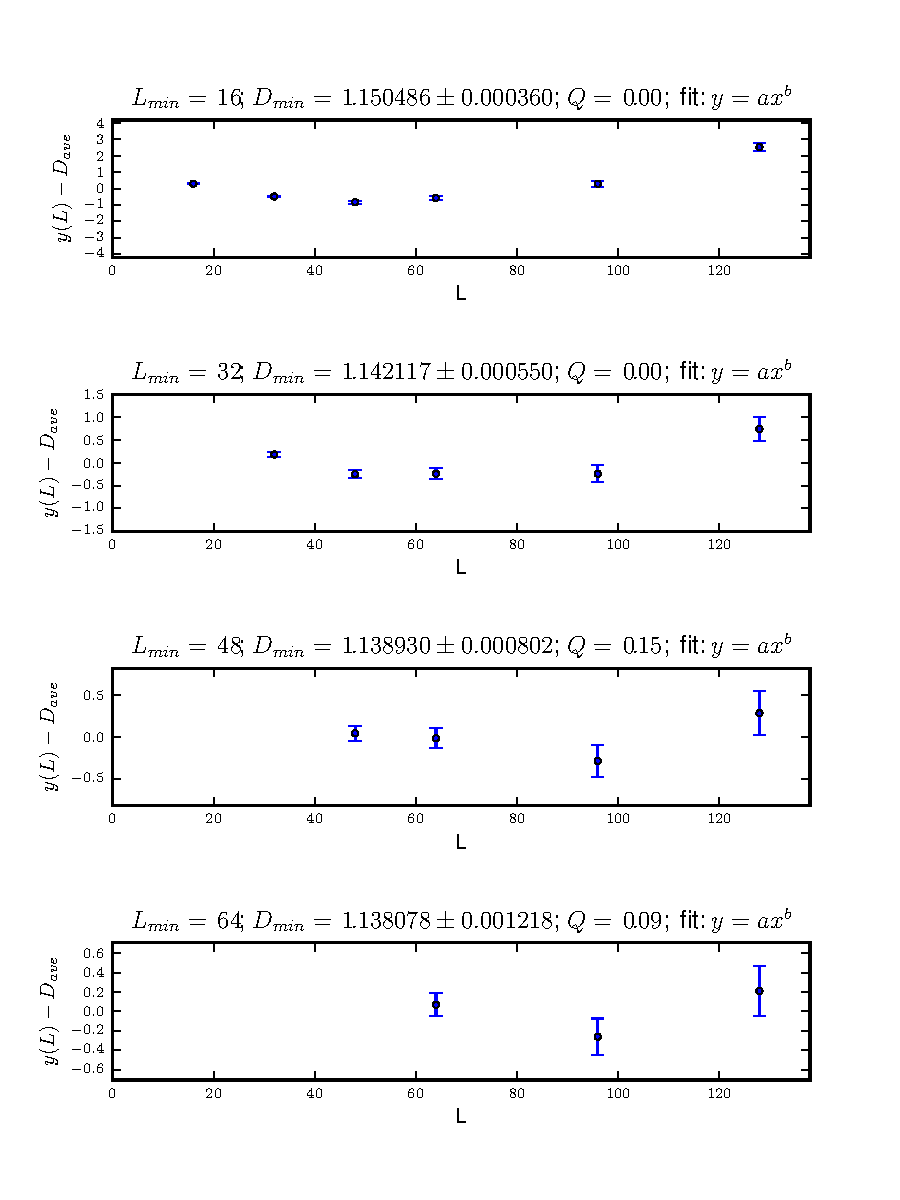
\includegraphics[width=.85\textwidth]{figures/d_min_D2q1_46_fig}
\caption{The difference between the fit, $y(L)=cL^{d_{min}}$, and the average chemical distance $\lb l \rb$ for dim=2, q=1.}\label{fig:a}
\end{figure}

%q=1, D

\begin{figure}[htp]
\centering
\includegraphics[width=.85\textwidth]{figures/D_min_D2q1_46_fig}
\caption{The difference between the fit, $y(L)=cL^{D_{min}}$, and the average diameter $\lb D \rb$ for dim=2, q=1.}\label{fig:2}
\end{figure}


%q=2, d

\begin{figure}[htp]
\centering
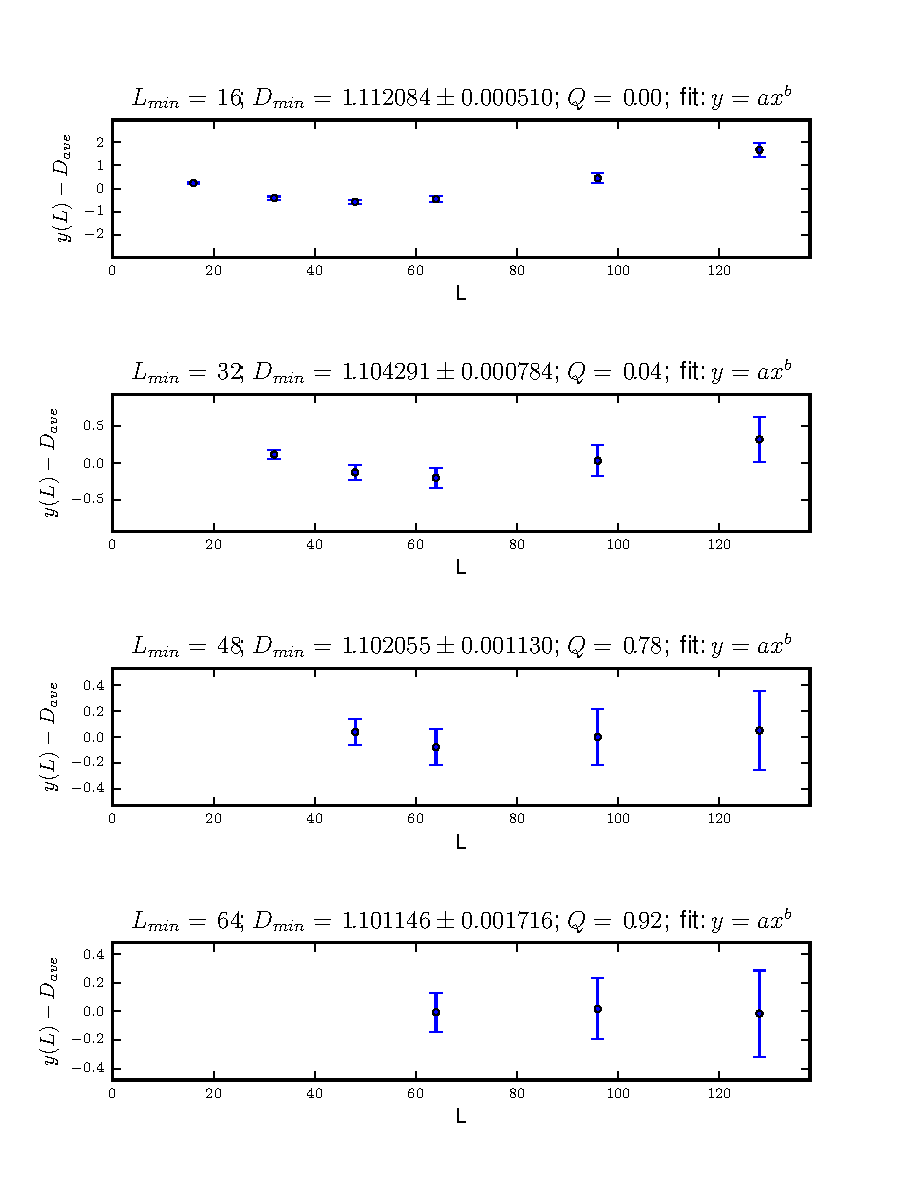
\includegraphics[width=.85\textwidth]{figures/d_min_D2q2_46_fig}
\caption{The difference between the fit, $y(L)=cL^{d_{min}}$, and the average chemical distance $\lb l \rb$ for dim=2, q=2.}\label{fig:3}
\end{figure}

%q=2, D

\begin{figure}[htp]
\centering
\includegraphics[width=.85\textwidth]{figures/D_min_D2q2_46_fig}
\caption{The difference between the fit, $y(L)=cL^{D_{min}}$, and the average diameter $\lb D \rb$ for dim=2, q=2.}\label{fig:4}
\end{figure}

%q=3, d

\begin{figure}[htp]
\centering
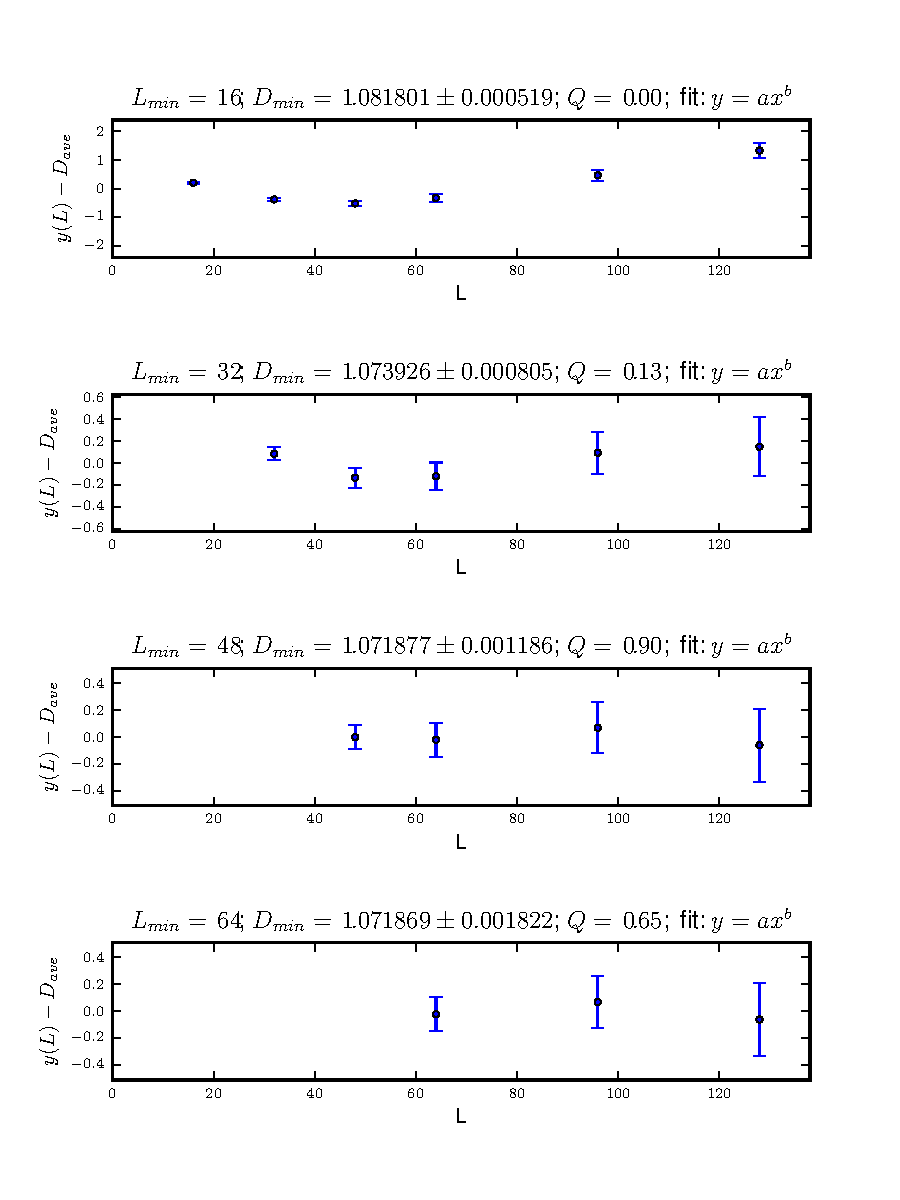
\includegraphics[width=.85\textwidth]{figures/d_min_D2q3_46_fig}
\caption{The difference between the fit, $y(L)=cL^{d_{min}}$, and the average chemical distance $\lb l \rb$ for dim=2, q=3.}\label{fig:4}
\end{figure}

%q=3, D

\begin{figure}[htp]
\centering
\includegraphics[width=.85\textwidth]{figures/D_min_D2q3_46_fig}
\caption{The difference between the fit, $y(L)=cL^{D_{min}}$, and the average diameter $\lb D \rb$ for dim=2, q=3.}\label{fig:4}
\end{figure}

%q=4, d

\begin{figure}[htp]
\centering
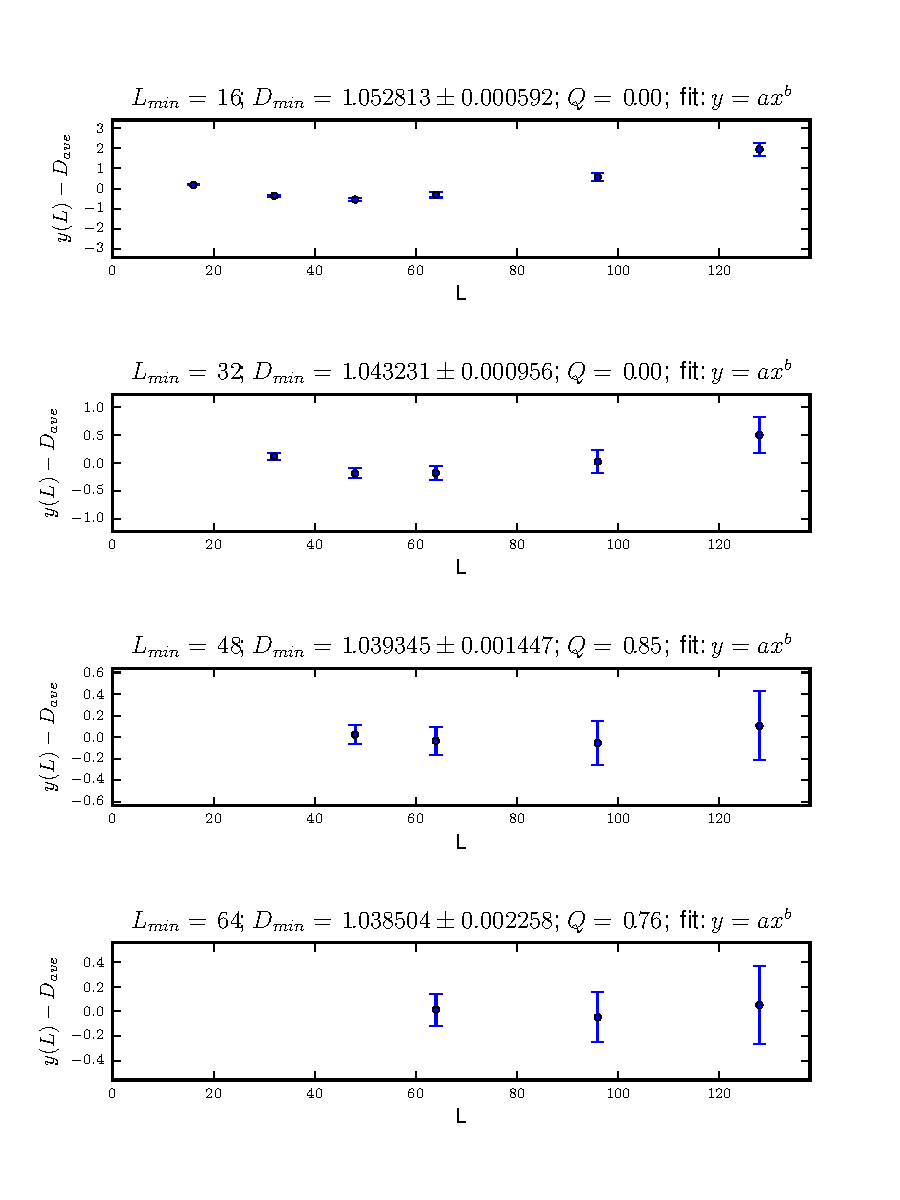
\includegraphics[width=.85\textwidth]{figures/d_min_D2q4_46_fig}
\caption{The difference between the fit, $y(L)=cL^{d_{min}}$, and the average chemical distance $\lb l \rb$ for dim=2, $q$=4.}\label{fig:4}
\end{figure}

%q=4, D

\begin{figure}[htp]
\centering
\includegraphics[width=.85\textwidth]{figures/D_min_D2q4_46_fig}
\caption{The difference between the fit, $y(L)=cL^{D_{min}}$, and the average diameter $\lb D \rb$ for dim=2, $q$=4.}\label{fig:4}
\end{figure}

%q=4, d, log fit

\begin{figure}[htp]
\centering
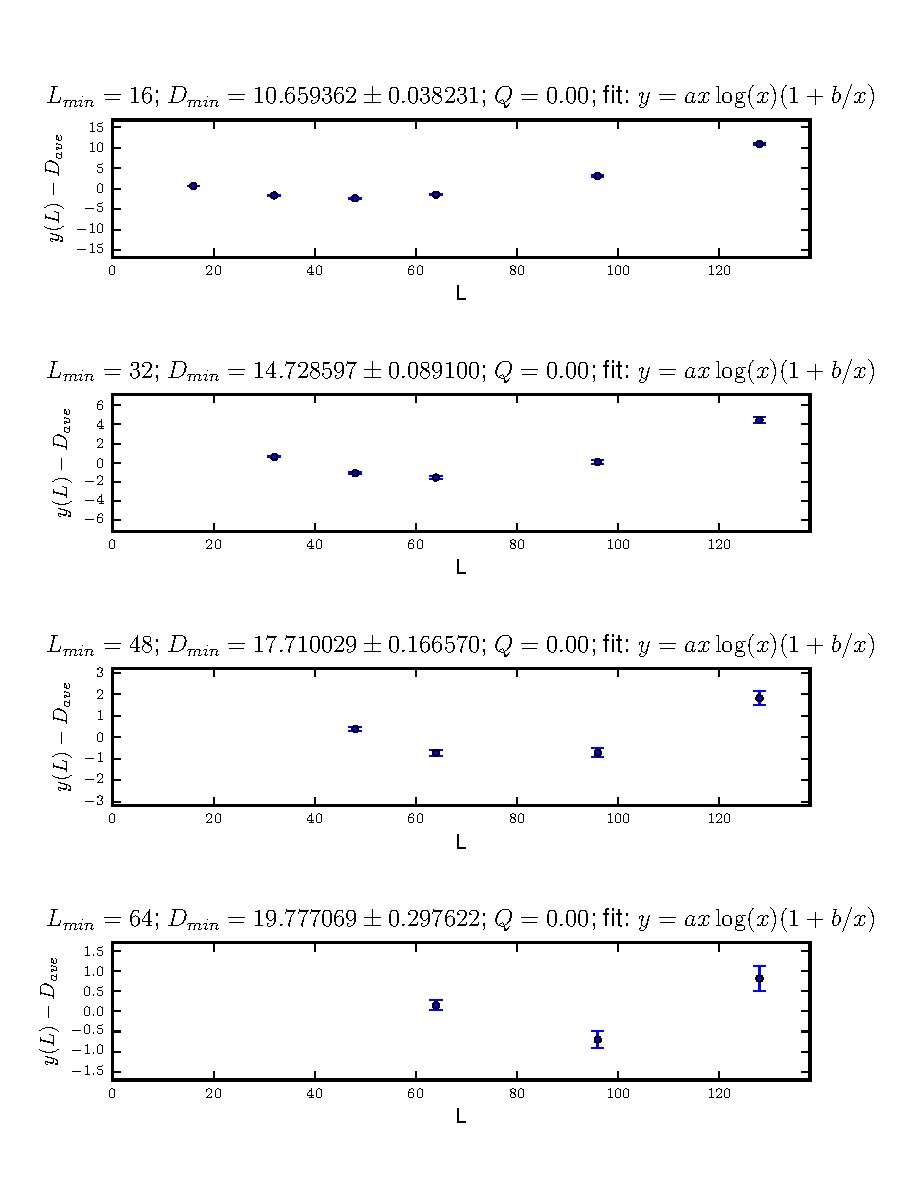
\includegraphics[width=.85\textwidth]{figures/d_min_D2q4_46_log_fig}
\caption{The difference between the fit, $y=AL\log{L}(1+B/L)$ and the average chemical distance, $\lb l \rb$ for dim=2, $q$=4.}\label{fig:4}
\end{figure}

%q=4, D, log fit

\begin{figure}[htp]
\centering
\includegraphics[width=.9\textwidth]{figures/D_min_D2q4_46_log_fig}
\caption{The difference between the fit, $y=AL\log{L}(1+B/L)$ and the average diameter, $\lb D \rb$ for dim=2, $q$=4.}\label{fig:4}
\end{figure}


%D=3, q=2

\begin{figure}[htp]
\centering
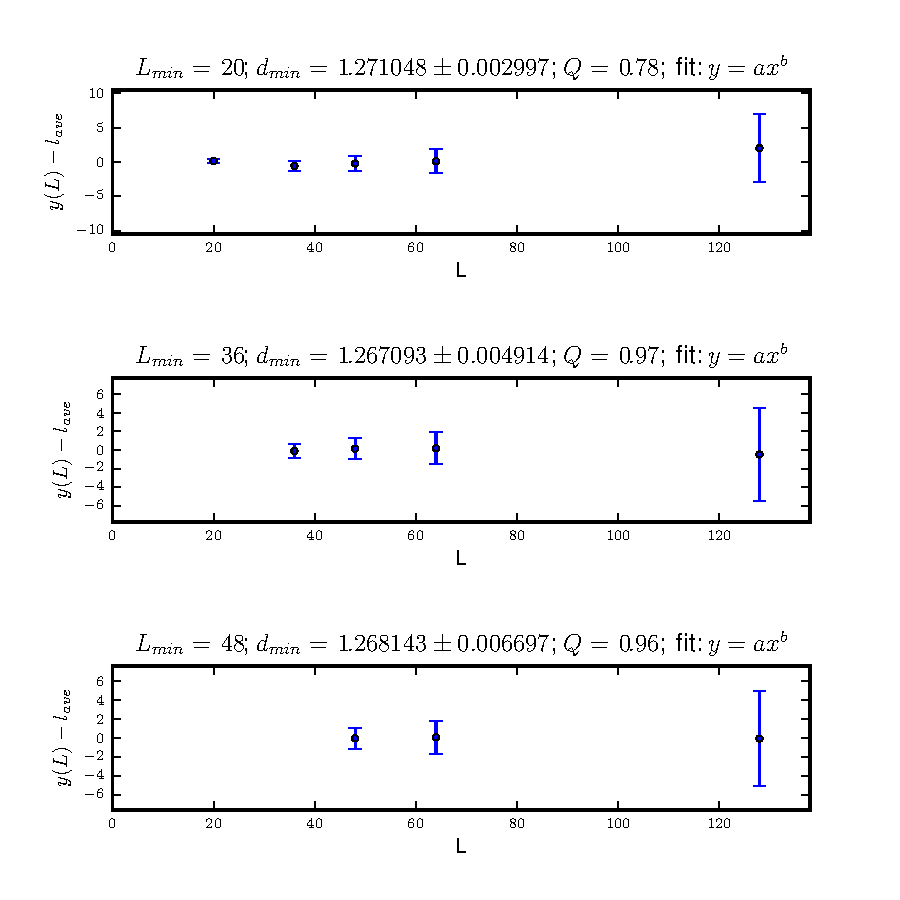
\includegraphics[width=.9\textwidth]{figures/d_min_D3q2_46_fig}
\caption{The difference between the fit, $y(L)=cL^{d_{min}}$, and the average diameter $\lb l \rb$ for dim=3, $q$=2.}\label{fig:4}
\end{figure}

%D=4, q=2

\begin{figure}[htp]
\centering
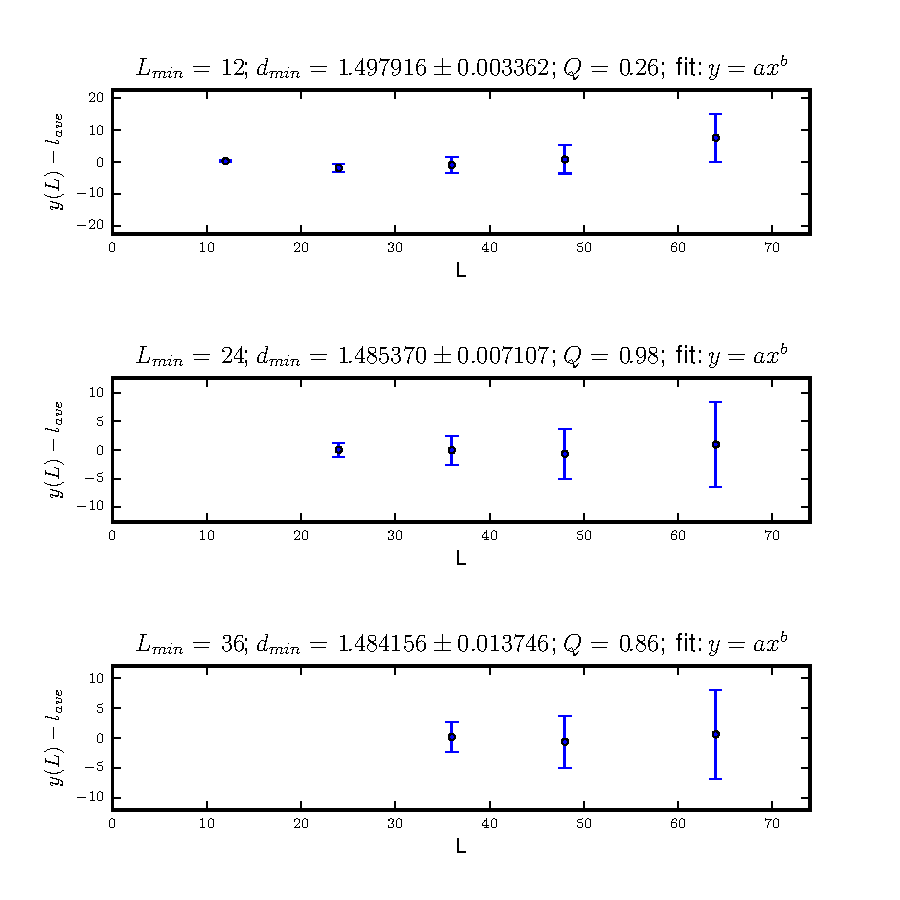
\includegraphics[width=.9\textwidth]{figures/d_min_D4q2_46_fig}
\caption{The difference between the fit, $y(L)=cL^{d_{min}}$, and the average diameter $\lb l \rb$ for dim=4, $q$=2.}\label{fig:b}
\end{figure}

\begin{figure}[htp]
\centering
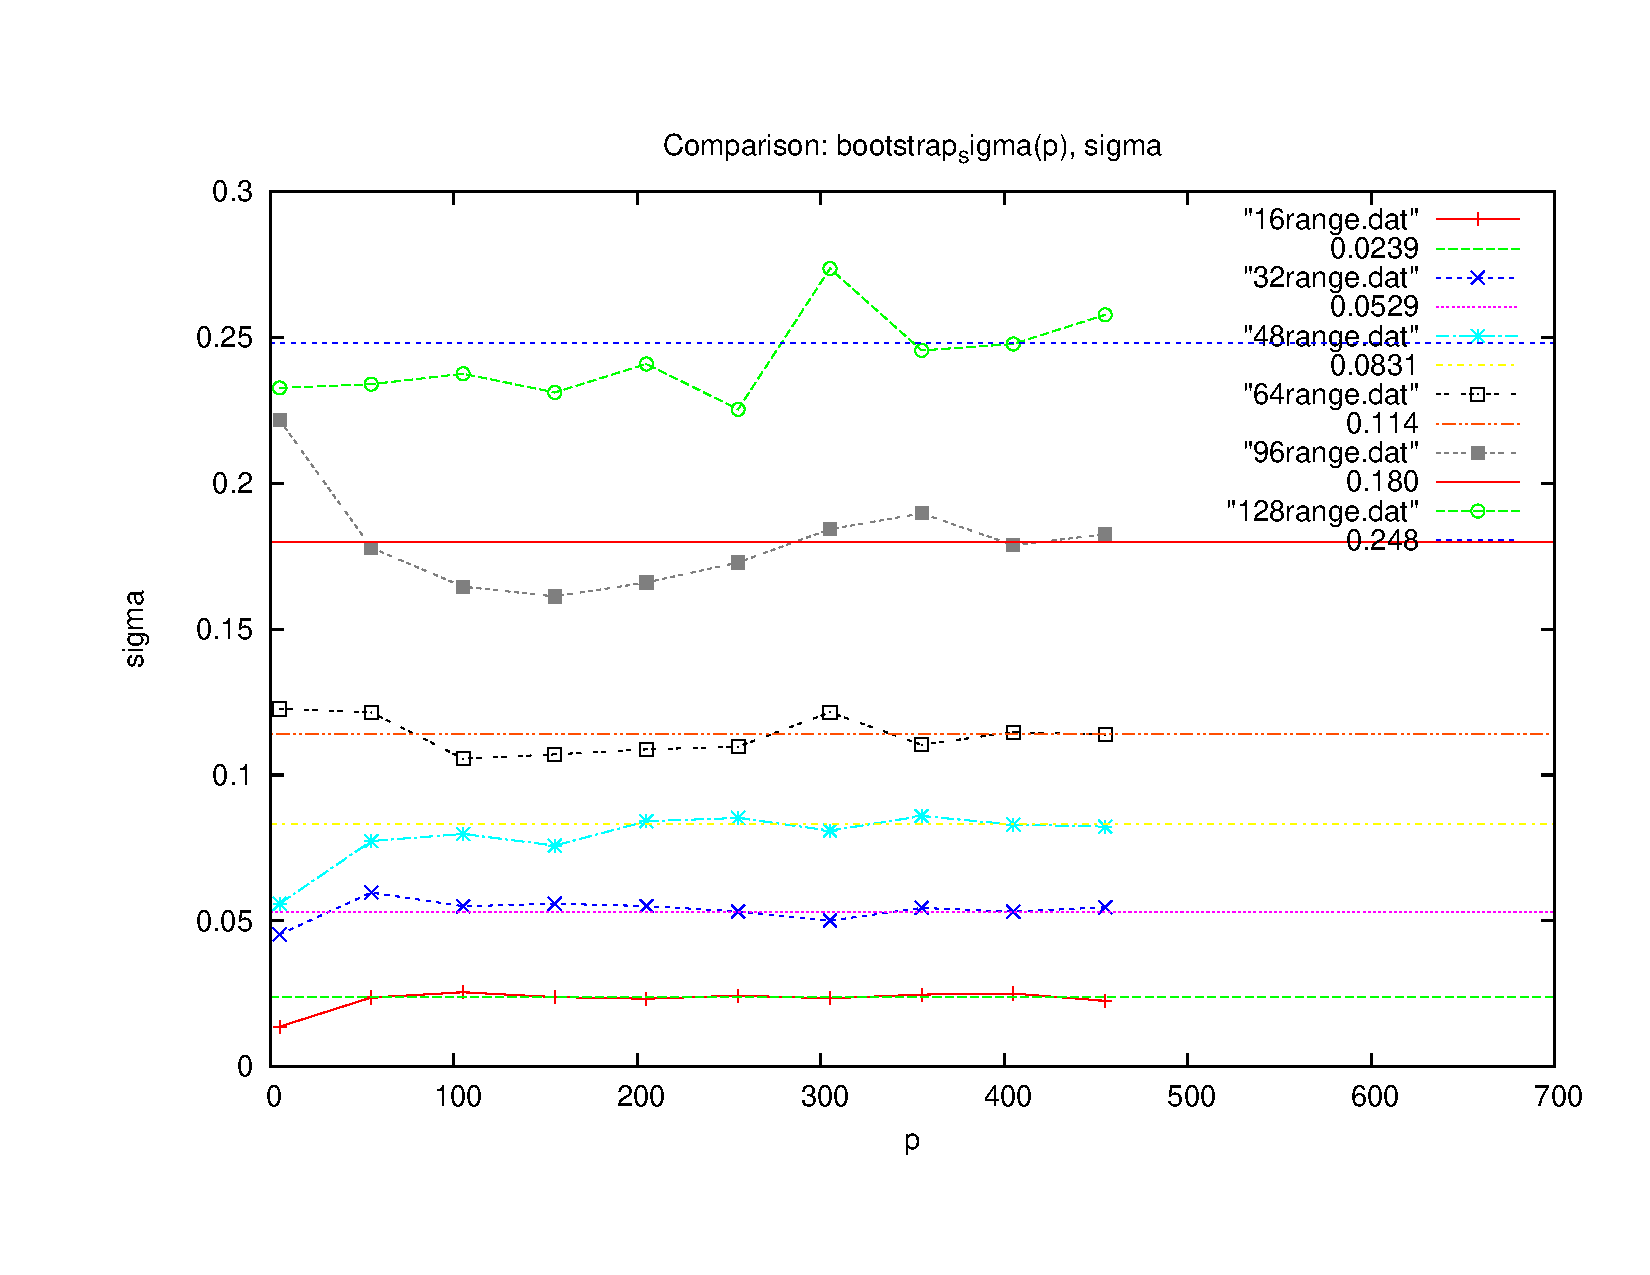
\includegraphics[width=.9\textwidth]{figures/boot}
\caption{$D=2, q=1, d_{min}$: comparison between $\sigma$ calculated as per the above description ``Methods'', and the bootstrap method with $p$ iterations.}\label{fig:b}
\end{figure}

\begin{figure}[htp]
\centering
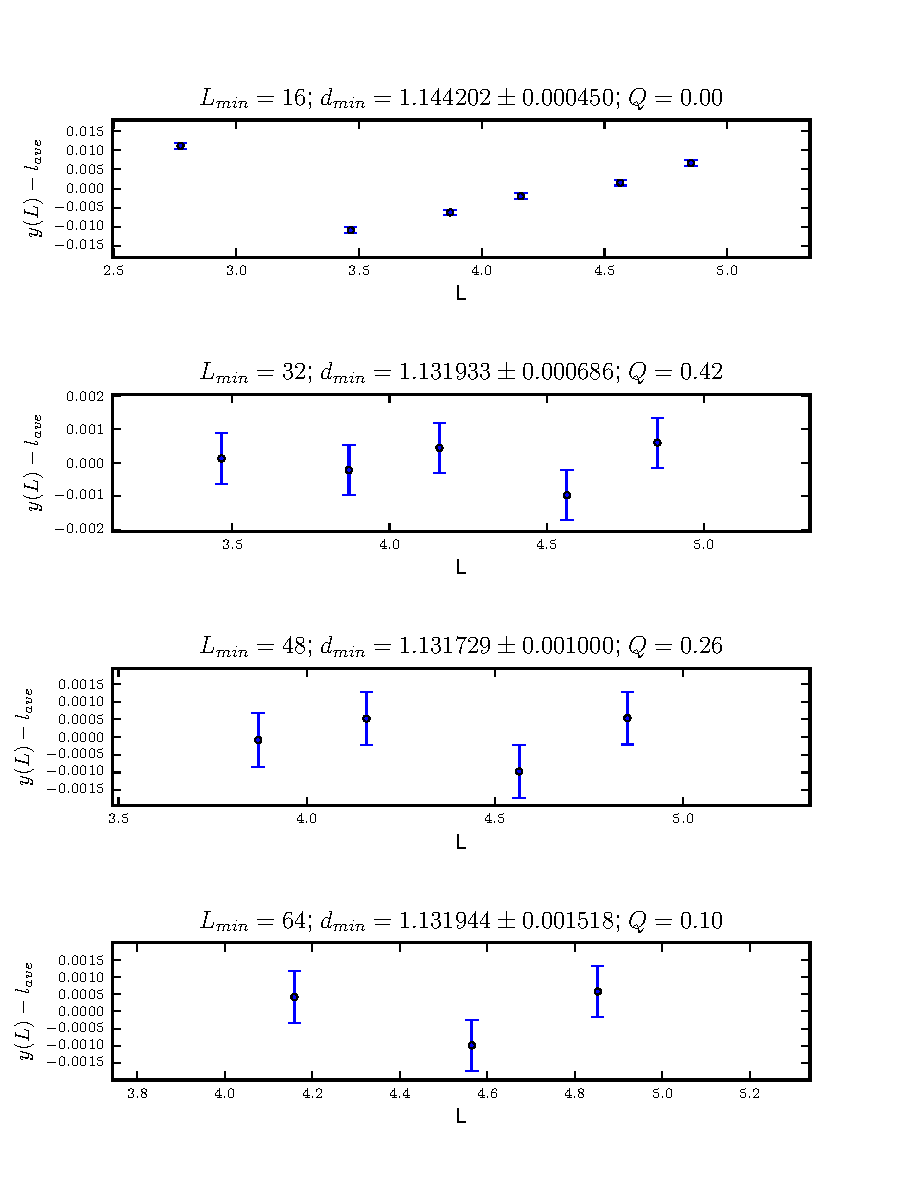
\includegraphics[width=.9\textwidth]{figures/d_min_D2q1_4601_fig_straightline}
\caption{$D=2, q=1, d_{min}$: linear fit of the ``log-log'' data (axes should be ``log'')}\label{fig:b}
\end{figure}

\begin{figure}[htp]
\centering
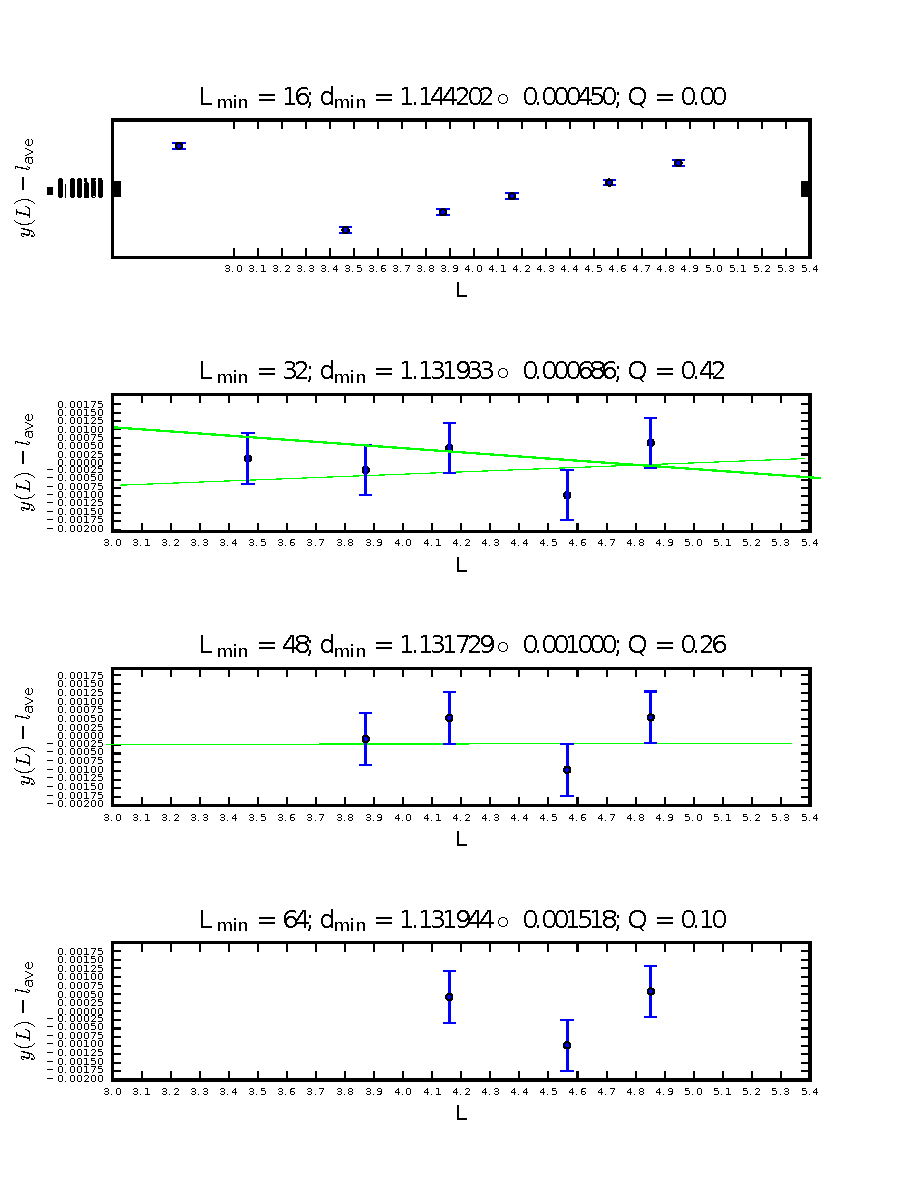
\includegraphics[width=.9\textwidth]{figures/d_min_D2q1_4601_fig_handfit_noboxes.pdf}
\caption{$D=2, q=1, L_{min}=32,d_{min}$: ``Hand-estimate'' of the error in the slope of the log-log data yields an error of $\pm 0.0010$ in the value for $d_{min}$ (axes should be ``log'').}\label{fig:b}
\end{figure}

\end{document}

